\subsection{Open loop stability}
\label{subsec:open_loop_stability}

The stability of the system can be assessed by analyzing the poles of the open-loop system, which corresponds to the eigenvalues of the system matrix $A$.
By solving the characteristic equation, we find that the poles of the system are located at:

\begin{equation}
    eig(A) =
    \begin{cases}
        39.44  \\
        -39.44 \\
        -35.56
    \end{cases}
\end{equation}

One can clearly notice that one of the poles is located on the right-hand side of the complex plane, indicating that the system is inherently unstable.

\paragraph{Root Locus}

Considering the unstable nature of the system, we perform a root locus analysis to identify potential proportional gains that achieve a stable closed-loop system.
The root locus plot is shown in Figure \ref{fig:root_locus_plot}.

\begin{figure}[H]
    \centering
    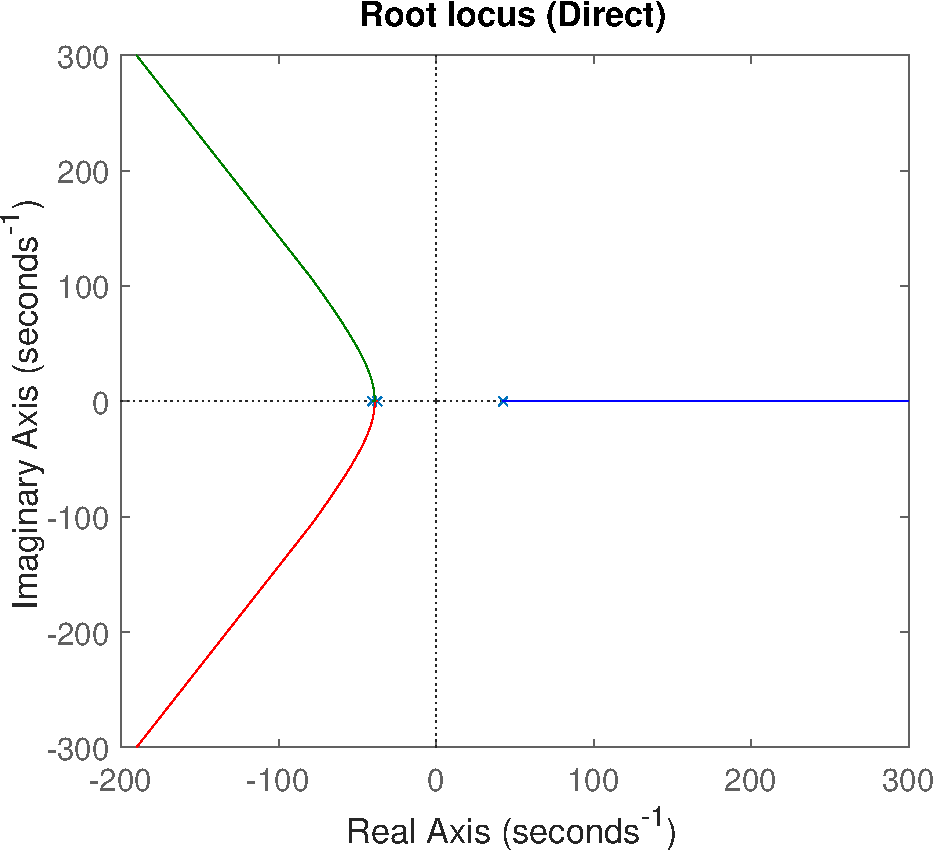
\includegraphics[width=0.47\textwidth]{./img/MATLAB/analysis/root_locus_direct.pdf}
    \hfill
    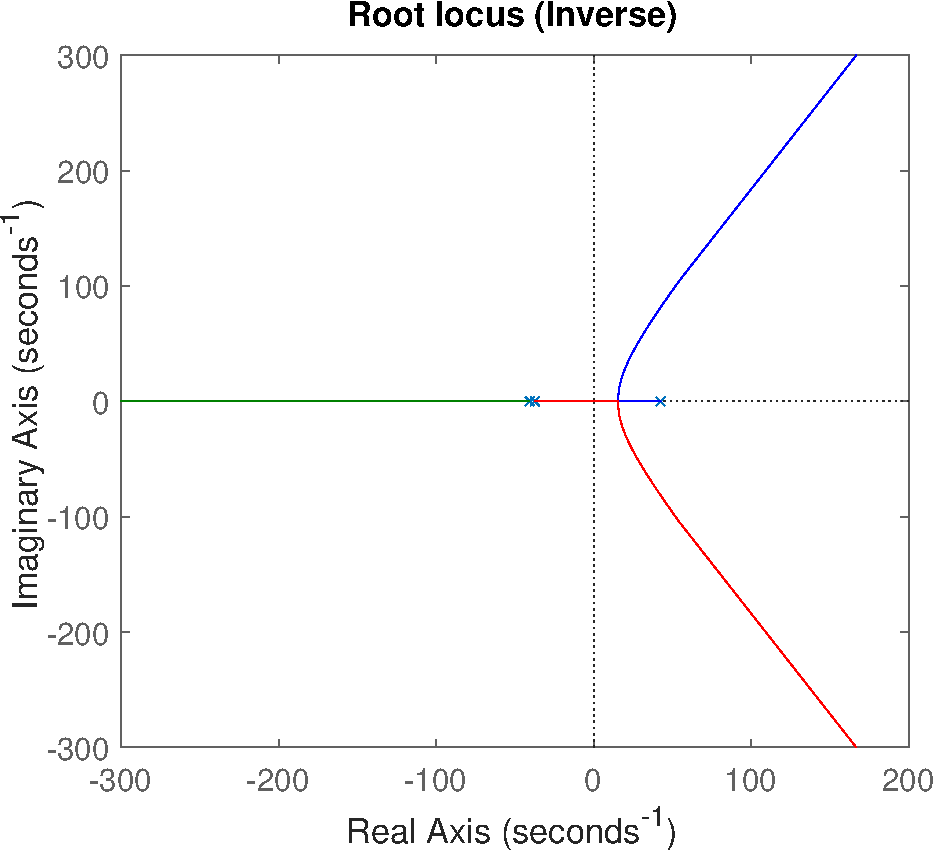
\includegraphics[width=0.47\textwidth]{./img/MATLAB/analysis/root_locus_inverse.pdf}
    \caption{Root Locus plot of the open loop system with direct and inverse proportional control.}
    \label{fig:root_locus_plot}
\end{figure}

The root locus plot illustrates how the system poles migrate in the complex plane as the proportional gain of the controller is varied.

Again, we observe that one the three poles is unstable, and we also notice that a simple proportional controller is not sufficient to stabilize the system, as the unstable poles do not move to the left-hand side of the complex plane for any value of the gain $K$.

\paragraph{Bode Diagram}

To further analyze the stability of the system, we consider the Bode plot for the open-loop transfer function.
The Bode diagram is shown in Figure \ref{fig:bode_plot}.

\begin{figure}[H]
    \centering
    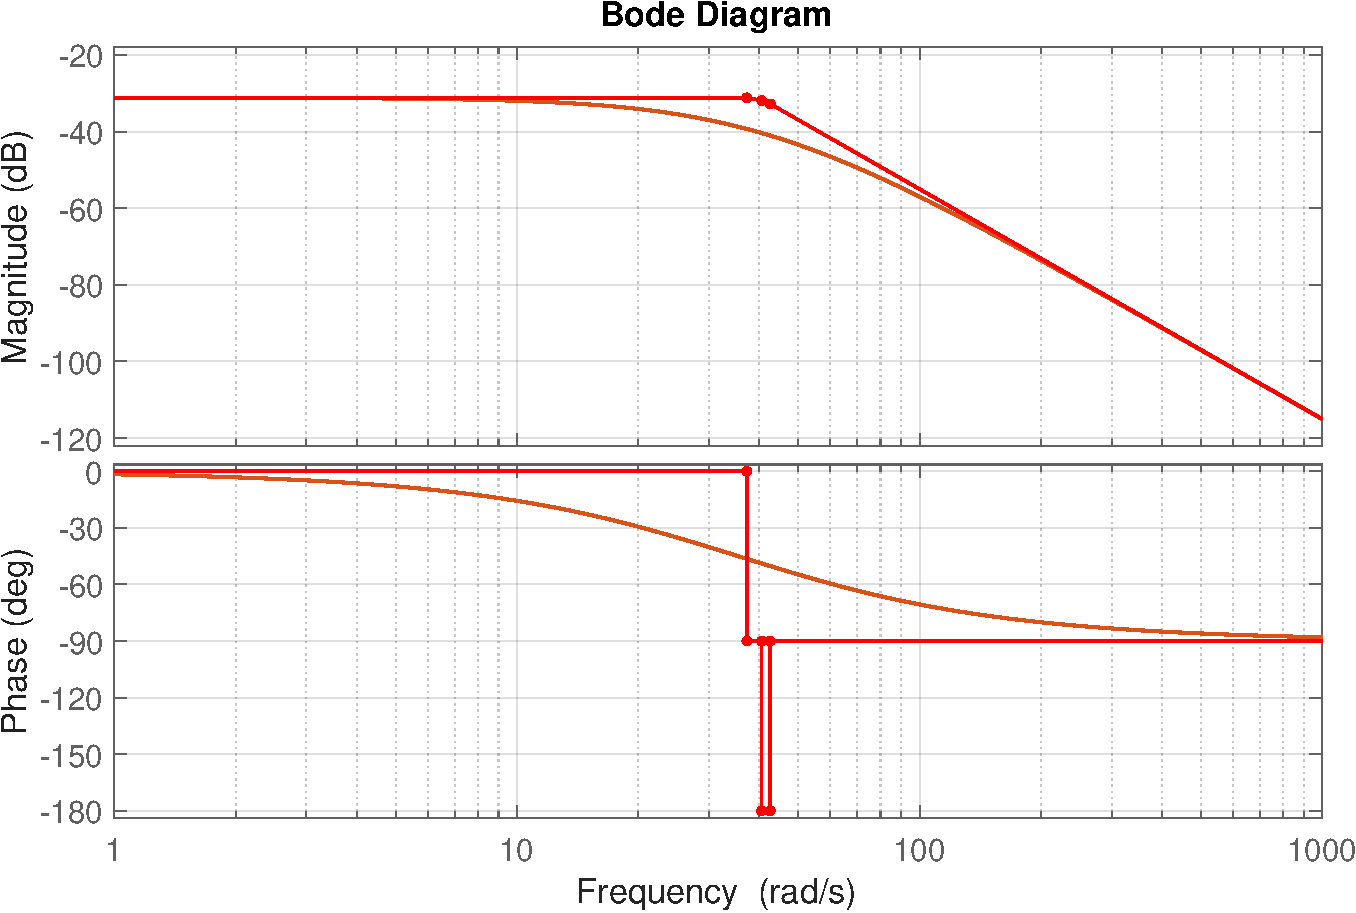
\includegraphics[width=0.8\textwidth]{./img/MATLAB/analysis/bode_plot.pdf}
    \caption{Bode plot of the open loop system.}
    \label{fig:bode_plot}
\end{figure}

Again, we observe that the system is unstable, as the gain margin is negative.